\chapter{Background and inspiration}

\section{Microcontrollers as alternative to computers}

When I joined MIT Media Lab in 2019, I made the decision to focus my efforts on hardware research, so I could make computational art devices, instead of software that needs to run on a laptop computer or a browser. This was fueled by the introduction of restrictive news by Apple, such as advising against the use of apps created by unregistered developers and discontinuing support for 32-bit apps, and by the ever-changing nature of the web, which makes my online artwork break often and need maintenance, and the need for additional corporate infrastructure to keep it online. In contrast I saw hardware as a space where I could deploy my ideas and keep them running without outside intervention.

I started my research by catching up with the newer developments by Teensy. The newer microcontrollers are faster and more powerful, and I used them to design and implement many small projects. I want to mention this personal project, a standalone audiobook I made with rotary encoders and a small screen for navigation, because it led me to include software for support of this same screen in the TinyTrainable library.

\begin{figure}[ht]
  \centering
  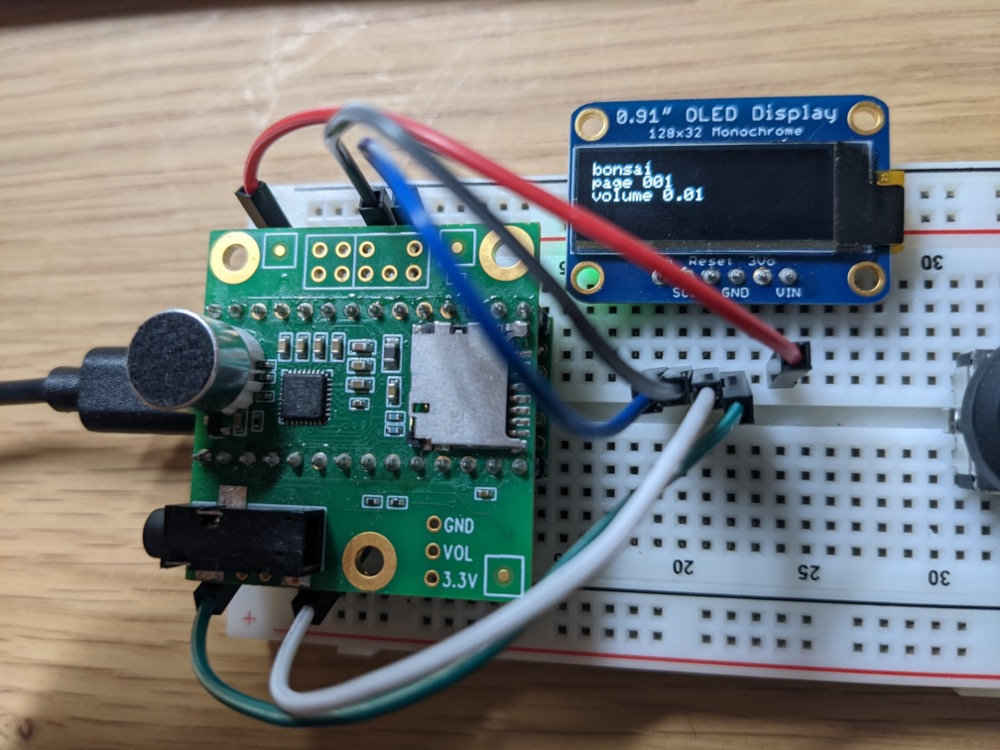
\includegraphics[width=0.75\linewidth,height=0.40\textheight,keepaspectratio]{images/bonsai.jpg}
  \caption{Audiobook made with Teensy}
  \caption*{Picture taken by myself}
  \label{fig:bonsai-audiobook}
\end{figure}

In parallel, I researched the evolution of the teaching of physical computing at \acrshort{NYU} \acrshort{ITP}, and I discovered that they stopped teaching with the now classic Arduino Uno, and have replaced it with the newer series of Arduino Nano microcontrollers, which have a smaller format and and operating voltage of 3.3V instead of 5V.

While browsing this series, I discovered the Arduino Nano 33 \acrshort{BLE} Sense that I based my thesis on. It comes with 9 embedded sensors, to measure and detect acceleration, movement, distance, color, plus a microphone. This is an amazing help for beginners, since a huge challenge when you are starting to build your own projects and learning electronics is reading datasheets to understand what sensors you can use with your microcontroller, how to wire them and calibrate them, and then what library supports it. This makes it easier and cheaper to prototype, and this made my work on my thesis easier, since I didn't have to include instructions for wiring sensors or calibrating them, and I could focus on \acrshort{ML} and the different outputs for arts.

\section{Coursework at MIT}

As part of the research that directly inspired this thesis, here is the coursework I took at MIT, and my notes about how they inform my theoretical and practical background for Tiny Trainable Instruments.

\begin{enumerate}
  \item Fall 2019, CMS.901 Current Debates in Media, by Professor Sasha Costanza-Chock
  \item Fall 2019, MAS.S65 Recreating The Past, by Professor Zach Lieberman
  \item Spring 2020, MAS.826 Sound: Past and Future, by Professor Tod Machover
  \item Spring 2020, MAS.712 Learning Creative Learning, by Professor Mitchel Resnick
\end{enumerate}

In the class Current Debates in Media, topics covered included fake news, surveillance, algorithmic bias, data colonialism, climate justice, algorithms of oppression, among others. For my final paper I wrote on the role of the media during the 2019 Chilean protests. This class directly inspired me to look for privacy-first \acrshort{ML}, and thinking about \acrshort{AI} in a critical way and not as clean safe automation, but as invisibilized labor, exploitation, and algorithmic bias and discrimination in the worst scenarios.

In the class Recreating the Past, I learned about media arts history, and I dived deep into the language C++ which I used for writing the TinyTrainable library, while working with the library openFrameworks, which is one of the most popular open source frameworks and communities for media arts.

In the class Sound: Past and Future, I learned more about the history of different computational advancements for sound, with a strong focus on projects at the MIT Media Lab's own research groups including Opera of the Future, Hyperinstruments, and Music, Mind, and Machine. This class introduced me to many projects and it helped me decide on making instruments for my thesis, using the latest technologies I could find, in this case, microcontrollers and \acrshort{ML}.

In the class Learning Creative Learning, I was introduced to the Lifelong Kindergarten's frameworks and ideas, including the 4 P's (projects, passion, peers, and play), and the design of Scratch as a home with low floor, wide walls, and high ceiling, which I highly recommend to follow up with  on Mitchel Resnick's book Lifelong Kindergarten \cite{lifelong-kindergarten}. This class gave me the push to write my software library with a community in mind, starting with the development of it. I made this happen by working with MIT undergrads Peter Tone and Maxwell Wang, who helped me with different aspects of research and development.

\subsection{TinyML Professional Certificate}

Apart from the MIT coursework, between November 2020 and March 2021 I completed the online Tiny Machine Learning Professional Certificate by Harvard University at the platform edx \cite{website-edx-harvardx-tinymlx-professional-certificate}. It is a series of three courses, where they teach responsible \acrshort{AI} strategies, theoretical \acrshort{ML}, and applied tiny \acrshort{ML} with the Arduino Nano 33 BLE Sense microcontroller, with a focus on industrial applications.

The academic team behind this certificate released the companion Harvard tinyMLx Arduino library \cite{repository-tinymlx-arduino-library}, which is based on the vanilla Arduino TensorFlowLite for microcontrollers. Through the example of this library, I learned how to build my own library for this thesis.

During this coursework I researched other libraries for machine learning, and discovered the Arduino \acrshort{k-NN} library \cite{repository-arduino-knn}. I included this library as a dependency on my thesis because it allows on-device data capture and model training. This allows for the data never leaving the device, and to enhance privacy, which is one of the driving concepts of this project.

\section{Research projects at MIT}

Another aspect of my research that I want to highlight is other research projects I worked on while at the MIT Media Lab, because they follow my same interests and passions, and I hope they help inform the process behind my thesis.

\subsection{SiguesAhi}

SiguesAhi \cite{website-library-siguesahi} (from the Spanish "Are you still there?") is an instrument to detect when oppressive institutions have ceased to exist. It is achieved with microcontrollers with internet connectivity.  I built it using a microcontroller from the same series and format but different architecture and capabilities, the Arduino Nano 33 IoT.

\begin{figure}[ht]
  \centering
  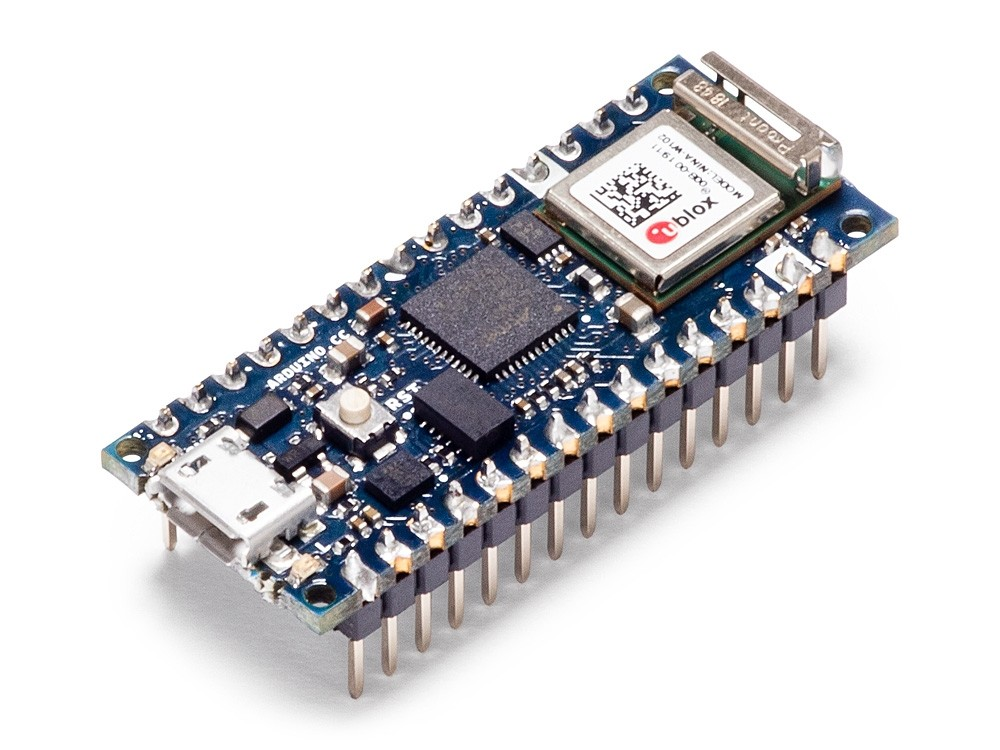
\includegraphics[width=0.75\linewidth,height=0.20\textheight,keepaspectratio]{images/arduino-nano-33-iot-with-headers.jpg}
  \caption{Arduino Nano 33 IoT with headers}
  \caption*{Retrieved from \cite{website-arduino-nano-33-iot-with-headers}}
  \label{}
\end{figure}

SiguesAhi's functionality is accomplished by connecting the microcontroller to the internet, and making it periodically download the first paragraph of the institution's Wikipedia article. Then the microcontroller checks if the first sentence is written in either present or past tense, and determines the existence of the institution. In the examples published in the alpha version of the software library \cite{website-library-siguesahi}, I am monitoring the National Rifle Association, which sadly still exists. 

\begin{figure}[ht]
  \centering
  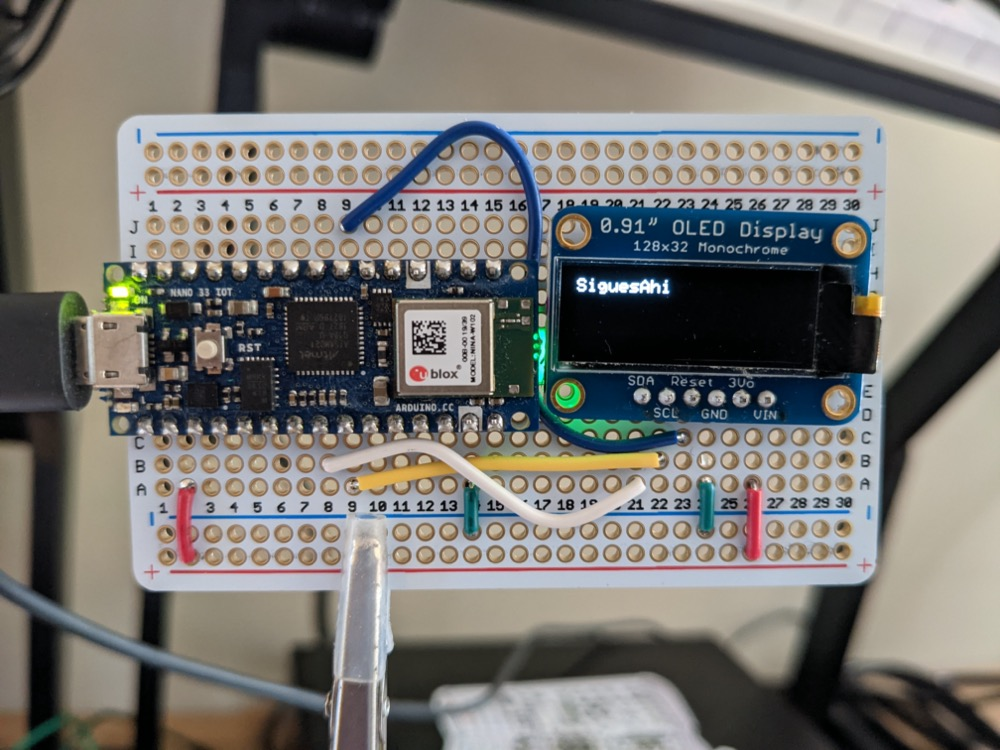
\includegraphics[width=0.75\linewidth,height=0.25\textheight,keepaspectratio]{images/siguesahi.jpg}
  \caption{SiguesAhi project}
  \caption*{Picture by myself}
  \label{fig:siguesahi}
\end{figure}

As a feature, I am adding support for Wikipedia articles in different languages, with the hope that people can use this library to make their own instruments to track the downfall of oppressive institutions wherever they are. I am building one for myself to track the existence of the current Chilean Constitution, written in 1980 by the military dictatorship.

SiguesAhi has been developed in parallel to Tiny Trainable Instruments, and has been possible thanks to the techniques and strategies I have learned about instrument making and publishing software libraries for arts.

\subsection{Open Drawing Machine}

The Open Drawing Machine \cite{website-open-drawing-machine} is a collaborative project with Gaurav Patekar for the research group Future Sketches at the MIT Media Lab. It is a low cost open source machine, consisting of an Arduino microcontroller and hardware for drawing computationally.

\begin{figure}[ht]
  \centering
  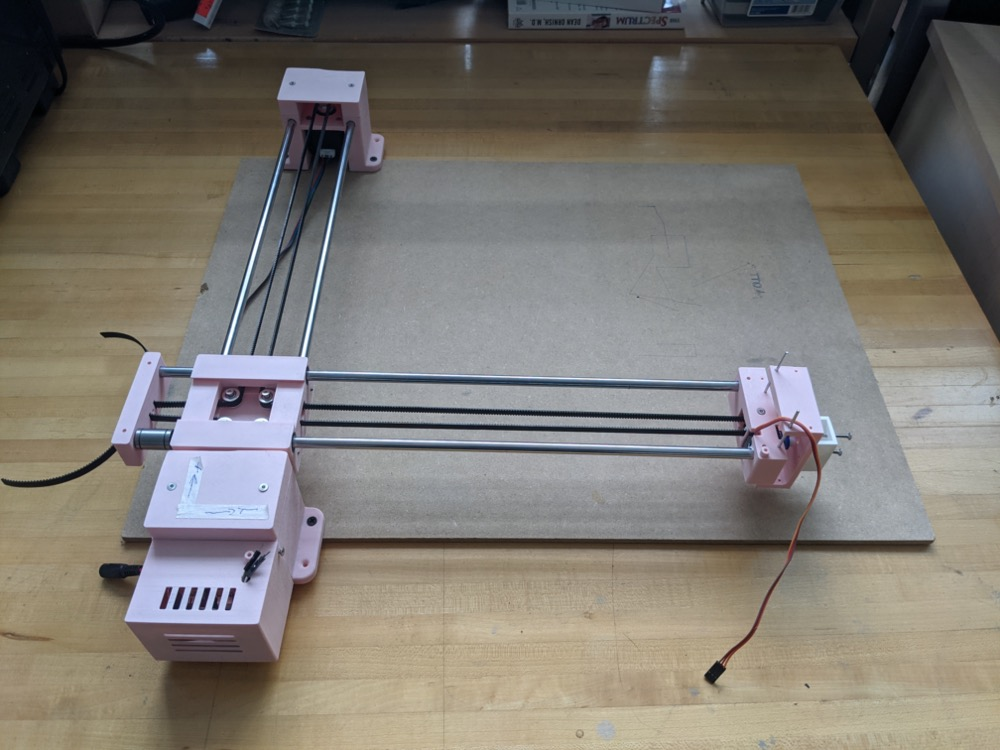
\includegraphics[width=0.75\linewidth,height=0.25\textheight,keepaspectratio]{images/open-drawing-machine.jpg}
  \caption{Open Drawing Machine project}
  \caption*{Picture by myself}
  \label{fig:open-drawing-machine}
\end{figure}

Gaurav Patekar designed and 3D-printed the hardware, and I packaged our code and published a library add-on for openFrameworks. Currently the Open Drawing Machine can receive drawing commands from a computer through a serial port, and the next step of this project is being able to receive commands from other computers through networks and the internet.

\subsection{Introduction to networks for artists}

Introduction to networks for artists \cite{website-intro-to-computer-networks-for-artists} is a series of tutorials for beginners, to learn how to set up their own networks and collaborate remotely in peer-to-peer ways for making art, featuring several open source software tools for arts. This project is inspired by the amazing research on remote collaboration, body sensors, peer-to-peer protocols, by movement artist and programmer Lisa Jamhoury \cite{website-lisa-jamhoury}, including the app Kinectron \cite{website-repository-kinectron}, to which I am a contributor.

\begin{figure}[ht]
  \centering
  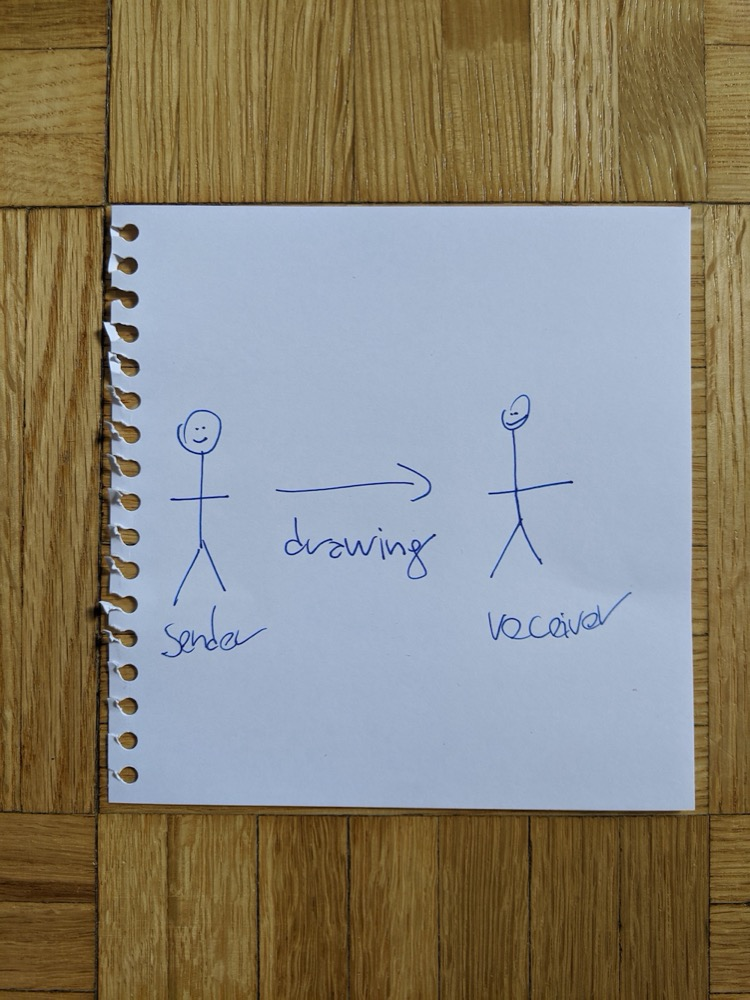
\includegraphics[width=0.75\linewidth,height=0.35\textheight,keepaspectratio]{images/intro-to-computer-networks-for-artists.jpg}
  \caption{Introduction to computer networks for artists project}
  \caption*{Picture by myself}
  \label{fig:intro-to-computer-networks-for-artists}
\end{figure}

\section{Computational media arts instruments}

A big concentration of my research at the MIT Media Lab is computational media arts instruments. I define them as devices that convert the data from an input like human gesture, to process and output different media (audio, video, text, light, etc), using digital operations.

Nowadays artists have access to a rich ecosystem of computers, operating systems and software for making art, and it is common for them to rely on their personal computer for making all of their art, on the go, wherever they are. In the 1990s, musicians stopped having to rely on analog hardware for recording and mixing, and broadly embraced digital technology, with a huge reduction in costs and maintenance.

In this section of my thesis I will share my research on companies making some of my favorite recent computational media arts instruments, with a strong focus on the ones that can be programmed, and that promote open source hardware or software. Many of these instruments often sit at my desk for inspiration, or I spend hours playing with them for my art and learning from them and the communities around them.

The tables \ref{table:media-arts-instruments-technical} and \ref{table:media-arts-instruments-influence} are respectively summaries of techniques and influences of the instruments that I reference in this section.

\begin{table}[ht]
    \centering
    \begin{tabular}{ | l |  l | l | l | l |}
        \hline
        \textbf{Company} & \textbf{Instrument} & \textbf{Year} & \textbf{Basis} & \textbf{Software} \\
        \hline
        Bastl Instruments   & Illuminati    & 2019  & MCU       & None                \\
        \hline
        Bastl Instruments   & Kastle Drum   & 2020  & MCU       & Arduino, C++        \\
        \hline
        Bastl Instruments   & Kastle v1.5   & 2017  & MCU       & Arduino, C++        \\
        \hline
        Bastl Instruments   & OMSynth       & 2016  & IC        & None                \\
        \hline
        Bastl Instruments   & microGranny 2 & 2016  & MCU       & Arduino, C++        \\
        \hline
        Bastl Instruments   & Servo         & 2016  & MCU       & Arduino, C          \\
        \hline
        Critter \& Guitari  & Organelle     & 2016  & Linux     & Pure Data           \\
        \hline
        Critter \& Guitari  & EYESY         & 2020  & Linux     & Python, Pygame      \\
        \hline
        monome              & aleph         & 2013  & Linux     & C                   \\
        \hline
        monome              & norns         & 2018  & Linux     & Lua, SuperCollider  \\
        \hline
        Shbobo              & Shnth         & 2013  & MCU       & Shlisp              \\
        \hline
        Shbobo              & Shtar         & 2017  & MCU       & Shlisp              \\
        \hline
    \end{tabular}
    \caption{Technical details of media arts instruments}
    \label{table:media-arts-instruments-technical}
\end{table}{}

\begin{table}[ht]
    \centering
    \begin{tabular}{ | l |  l | l |}
        \hline
        \textbf{Company}    & \textbf{Instrument} & \textbf{Influence}              \\
        \hline
        Bastl Instruments   & Illuminati    & Output with LEDs                      \\
        \hline
        Bastl Instruments   & Kastle series & Use of breadboard and jumper wires    \\
        \hline
        Bastl Instruments   & OMSynth       & Distribution as tutorials + parts kit \\
        \hline
        Bastl Instruments   & microGranny 2 & Arduino as basis for instrument       \\
        \hline
        Bastl Instruments   & Servo         & Output with servo motor               \\
        \hline
        Critter \& Guitari  & Organelle     & Scriptable audio computer             \\
        \hline
        Critter \& Guitari  & ETC, EYESY    & Scriptable visuals computer, screen output\\
        \hline
        monome              & aleph, norns  & Scriptable audio computer            \\
        \hline
        Shbobo              & Shnth, Shtar  & Multiple input sensors, scripting     \\
        \hline
    \end{tabular}
    \caption{Influence of media arts instruments}
    \label{table:media-arts-instruments-influence}
\end{table}{}

\subsection{Bastl Instruments}

Bastl Instruments is a Czech company of multimedia instruments, which has had a huge impact and influence on my research and practice. When I first started researching the Eurorack format some years ago, I visited the shop Control in Brooklyn, NY, and some modules by Bastl stood out to me, because of their wooden panels and interaction with classic physical computing educational materials, such as motors and solenoids, which was an inspiration for me to include servo motors as an output option in the Tiny Trainable Instruments.

\begin{figure}[ht]
  \centering
  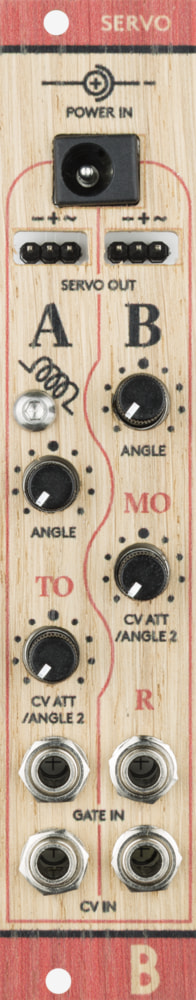
\includegraphics[width=0.75\linewidth,height=0.25\textheight,keepaspectratio]{images/bastl-servo.jpg}
  \caption{Bastl Instruments Servo module}
  \caption*{Retrieved from \cite{website-bastl-instruments-current}}
  \label{fig:bastl-servo}
\end{figure}

Another inspiration comes from their microGranny 2 granular sampler which is made with an Atmega microcontroller and its firmware is open source and available as a repository on their GitHub account \cite{github-bastl-instruments}, along with many other of their instruments.

\begin{figure}[ht]
  \centering
  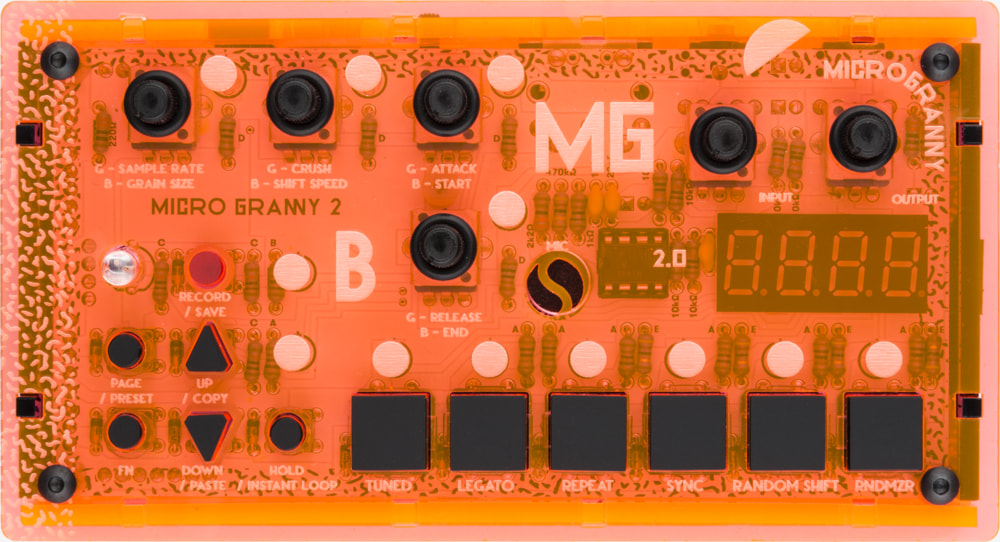
\includegraphics[width=0.75\linewidth,height=0.25\textheight,keepaspectratio]{images/bastl-microgranny-2.jpg}
  \caption{Bastl Instruments microGranny 2}
  \caption*{Retrieved from \cite{website-bastl-instruments-current}}
  \label{fig:bastl-microgranny-2}
\end{figure}

Their Kastle synthesizers are also based on microcontrollers, and feature a patchbay for making connections with jumper wires, the same used for prototyping in electronic breadboards. This influenced me to build the Tiny Trainable Instruments with breadboards and jumper wires, instead of custom \acrshortpl{PCB}.

\begin{figure}[ht]
  \centering
  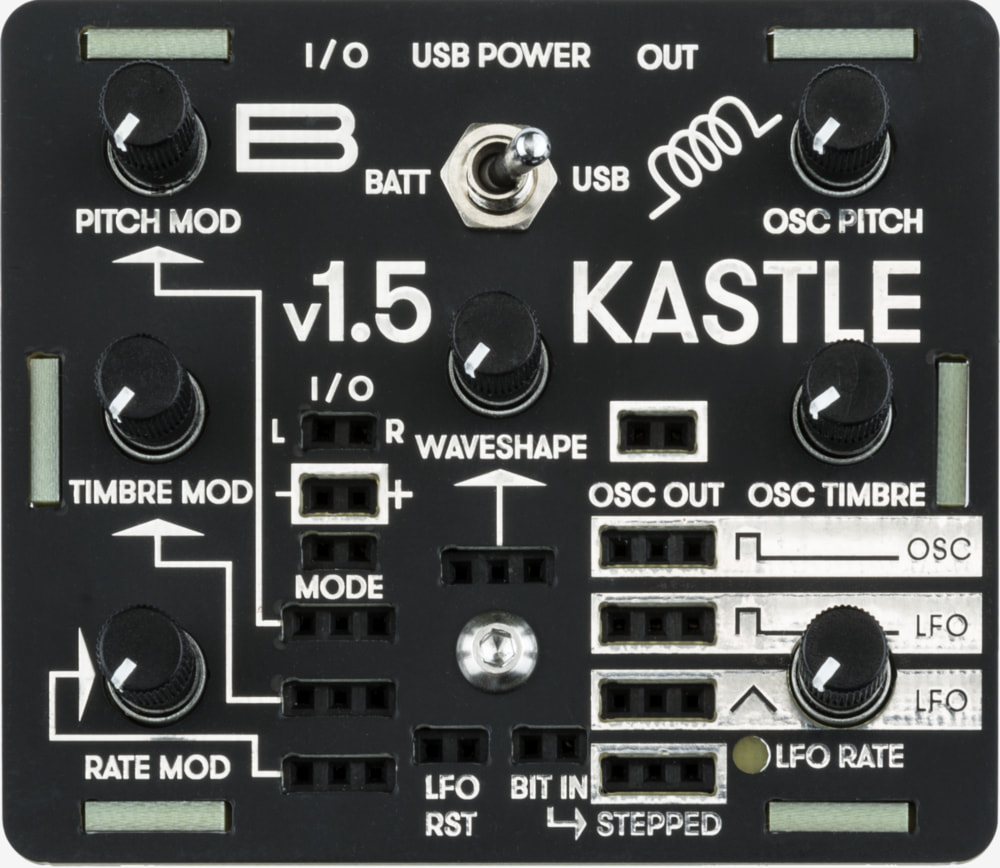
\includegraphics[width=0.75\linewidth,height=0.25\textheight,keepaspectratio]{images/bastl-kastle-v15.jpg}
  \caption{Bastl Instruments Kastle v1.5}
  \caption*{Retrieved from \cite{website-bastl-instruments-current}}
  \label{fig:bastl-kastle-v15}
\end{figure}

Also, the Kastle synths are forgiving instruments, their inputs and outputs are robust enough to allow for mistakes in connections, in an electrical and mechanical way, which I think is perfect for safe experimentation. It would be a bummer if the instrument was easy to break, or if it demanded a huge effort in understanding electronics for using it. 

As of writing, two different units are in production, both retailing for around 100.00 USD: the Kastle v1.5 melodic / drone synthesizer, and the Kastle Drum, for rhythm. The only difference between these synthesizers is the firmware and the labels on the faceplate. The community is encouraged to write new firmware to modify their behavior. 

\begin{figure}[ht]
  \centering
  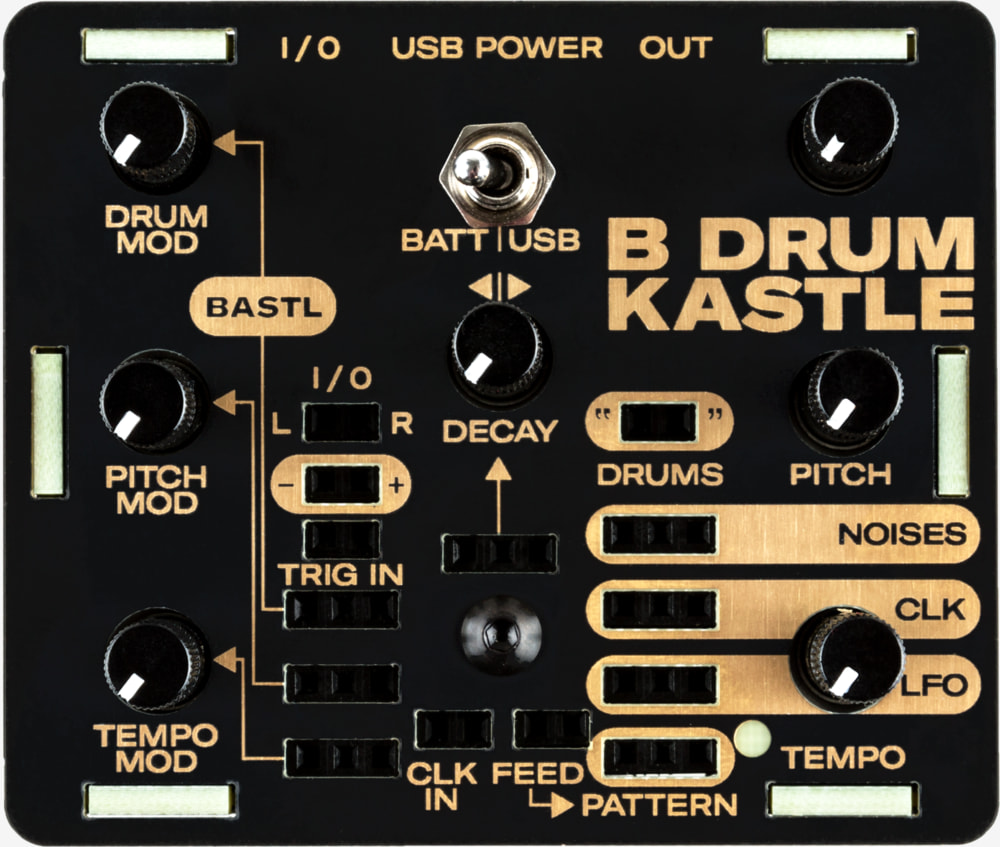
\includegraphics[width=0.75\linewidth,height=0.25\textheight,keepaspectratio]{images/bastl-kastle-drum.jpg}
  \caption{Bastl Instruments Kastle Drum}
  \caption*{Retrieved from \cite{website-bastl-instruments-current}}
  \label{fig:bastl-kastle-drum}
\end{figure}

Another instrument I want to highlight is the Illuminati, currently discontinued, a device that uses different inputs (audio, control voltage, \acrshort{MIDI} messages) to control the light intensity of connected USB lamps, which influenced the conception of Tiny Trainable Instruments as multimedia arts instruments, not only focusing on audio and music, but also printed text, light, and screen output.

\begin{figure}[ht]
  \centering
  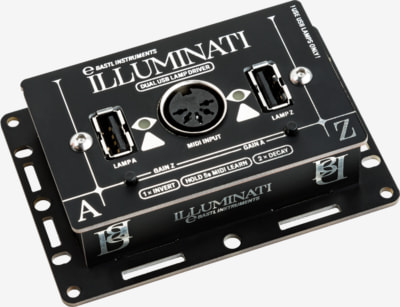
\includegraphics[width=0.75\linewidth,height=0.25\textheight,keepaspectratio]{images/bastl-illuminati.jpg}
  \caption{Bastl Instruments Illuminati}
  \caption*{Retrieved from \cite{website-bastl-instruments-current}}
  \label{fig:bastl-illuminati}
\end{figure}

The final instrument from this company that I want to highlight is the OMSynth, one of Bastl Instruments' many collaborations with Casper Electronics. This device is an educational and maker circuit development tool for creating synthesizers. It includes basic fundamental blocks, such as battery power, audio input and output, potentiometers for attenuating and boosting signals, and a suite of parts kits for building devices including sequencers, oscillators, and samplers, on the included breadboard. Its release as a kit was also a direct influence on the kits I designed for the workshops I taught with the Tiny Trainable Instruments.

\begin{figure}[ht]
  \centering
  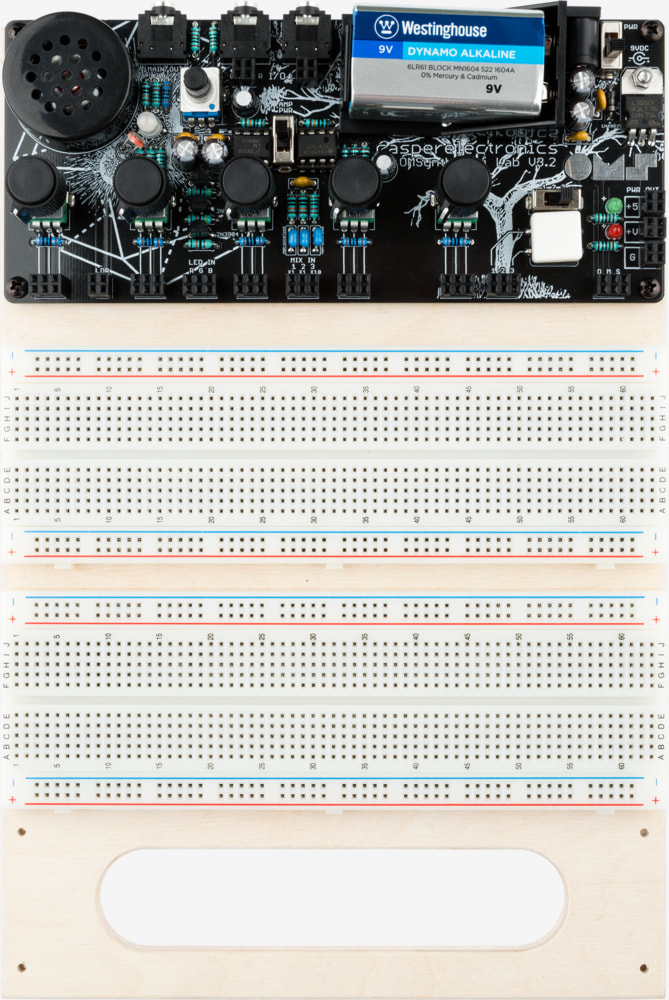
\includegraphics[width=0.75\linewidth,height=0.25\textheight,keepaspectratio]{images/bastl-omsynth.jpg}
  \caption{Bastl Instruments OMSynth}
  \caption*{Retrieved from \cite{website-bastl-instruments-current}}
  \label{fig:bastl-omsynth}
\end{figure}

Many Bastl standalone instruments are 200.00 USD or less, which is a huge contrast to the 1960s, when a Moog analog system II cost 6,200.00 USD, which was enough to buy a small house \cite{analog-days}. Also, many of their instruments are sold as kits for building and soldering them yourself, for the cheaper cost and the added educational aspect of having hands-on experience.

\subsection{Critter \& Guitari}

Critter \& Guitari is an American company based in Brooklyn, NY, which has released several computational microcontroller-based audiovisual instruments, from which my favorite is the currently discontinued Kaleidoloop. It is a sampler with an internal speaker and an included microphone, that allows you to record and playback audio. The instrument features two knobs for controlling the volume and playback rate of audio loops from your recordings. I really admire its portability, in terms of its size, weight, and being battery-powered, encouraging the recording and making of music while walking or in the park. This was a major influence on the design of the Tiny Trainable Instruments; the materials I picked are intended for building standalone instruments that you can power with a USB power bank or a battery, so that you can take them for a walk too.

\begin{figure}[ht]
  \centering
  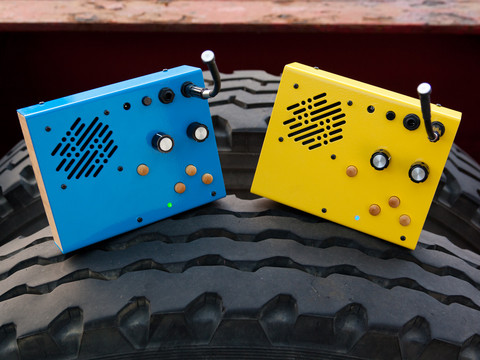
\includegraphics[width=0.75\linewidth,height=0.25\textheight,keepaspectratio]{images/critter-and-guitari-kaleidoloop.jpg}
  \caption{Critter \& Guitari Kaleidoloop}
  \caption*{Retrieved from \cite{website-critter-and-guitari-kaleidoloop}}
  \label{fig:critter-and-guitari-kaleidoloop}
\end{figure}

In 2015, Critter \& Guitari released the Organelle, a sound computer running the Linux operating system, and the \acrfull{Pd} software for programming patches that reacts to the computer's interface (knobs, encoders, keys), and then generates sound. It is currently on its second iteration, called Organelle M, with added features, such as an embedded speaker and microphone.

\begin{figure}[ht]
  \centering
  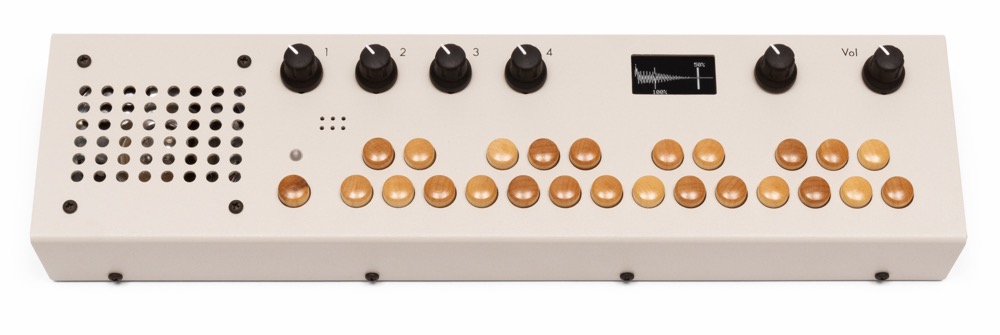
\includegraphics[width=0.75\linewidth,height=0.25\textheight,keepaspectratio]{images/critter-and-guitari-organelle-m.jpg}
  \caption{Critter \& Guitari Organelle M}
  \caption*{Retrieved from \cite{website-critter-and-guitari-current}}
  \label{fig:critter-and-guitari-organelle-m}
\end{figure}

Since the sound generation is made with the software \acrshort{Pd}, you can achieve the same sonic results on an Organelle or on your personal computer. Despite this, I am convinced that the Organelle is a revolutionary instrument,  because it allows artists to use computation in a single-purpose and stable device for their sound, in heavy contrast with the over-bloated personal computers we use from activities ranging from watching movies to paying taxes, and which constantly require updates and maintenance. The Organelle also replaces the keyboard and mouse in computers with an interface tailored for contemporary music production, including a musical keyboard for playing notes, knobs and encoders for changing parameters, and a screen for navigating menus.

The final aspects I want to celebrate about the Organelle are its ever growing capabilities, and the community behind it: Critter \& Guitari regularly publishes new \acrshort{Pd} patches, and the community also organizes in forums and repositories to share their creations. You don't need to be a programmer to enjoy the Organelle, you can download and use the new presets without ever having to open a code editor.

After the release of the Organelle, this company released the ETC visuals computer. It also runs the Linux operating system, and it uses the pygame Python library for generating graphics which can then be projected on a screen.  The ETC was discontinued and replaced with the EYESY, with upgrades such as a new mode for running openFrameworks.

\begin{figure}[ht]
  \centering
  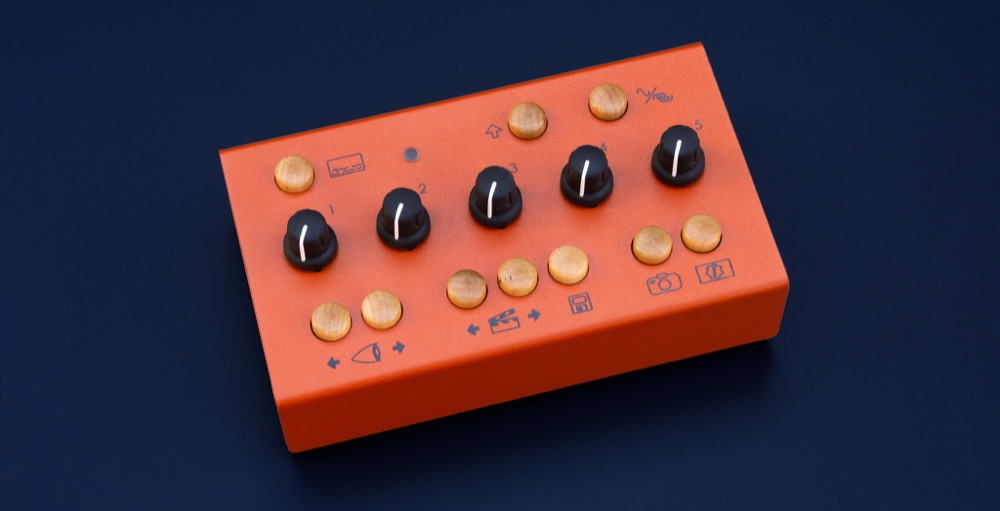
\includegraphics[width=0.75\linewidth,height=0.25\textheight,keepaspectratio]{images/critter-and-guitari-eyesy.jpg}
  \caption{Critter \& Guitari EYESY}
  \caption*{Retrieved from \cite{website-critter-and-guitari-current}}
  \label{fig:critter-and-guitari-eyesy}
\end{figure}

The current lineup of the Organelle and EYESY computers for arts make Critter \& Guitari a pioneering company in the creation of scriptable instruments that run open source software and foster communities around them. Tiny Trainable Instruments is heavily indebted to the work of this company, trying to promote scripting for microcontrollers for a new generation of artists.

\subsection{monome}

monome \cite{website-monome-current} is an American company based in upstate New York. Their first instrument was the grid, still in production. In its current iteration, it consists of 128 backlit silicone keys distributed in 8 rows and 16 columns. It has a USB port, through which it can be connected to all sorts of devices, including computers and Eurorack modules.

\begin{figure}[ht]
  \centering
  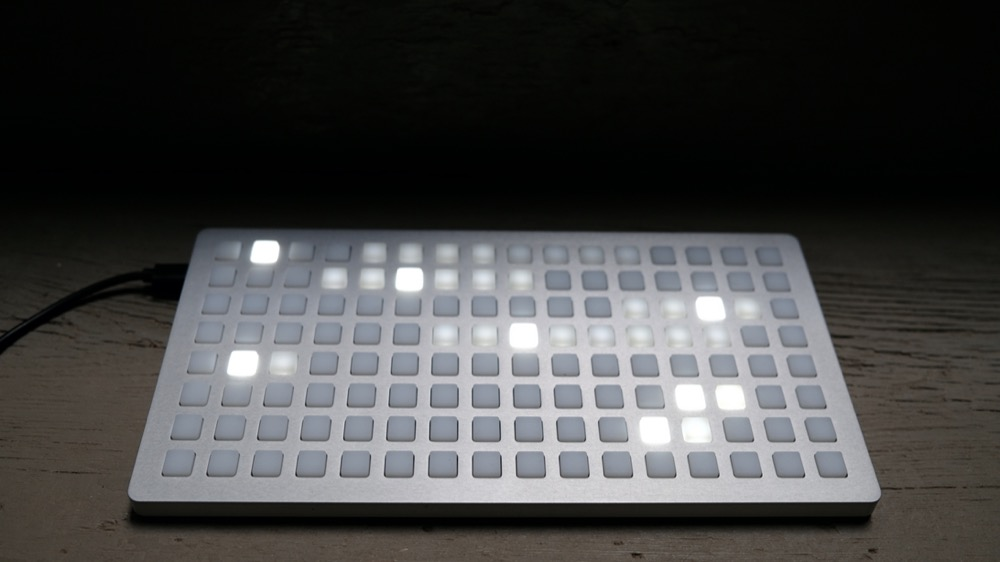
\includegraphics[width=0.75\linewidth,height=0.25\textheight,keepaspectratio]{images/monome-grid.jpg}
  \caption{monome grid}
  \caption*{Retrieved from \cite{website-monome-current}}
  \label{fig:monome-grid}
\end{figure}

The monome website features extensive tutorials for learning how to interface the grid with many popular open source hardware and software systems, including Arduino, Processing, \acrshort{Pd}, SuperCollider, Python, and Node.js. Over the years I have learned many important lessons about instrument making, software for arts, and live performance with my grid, and I am including what I learned on this thesis project.

Through the grid, I learned about the other instruments by monome, and I want to highlight the open source sound computers they have released, starting with the now-discontinued aleph.

\begin{figure}[ht]
  \centering
  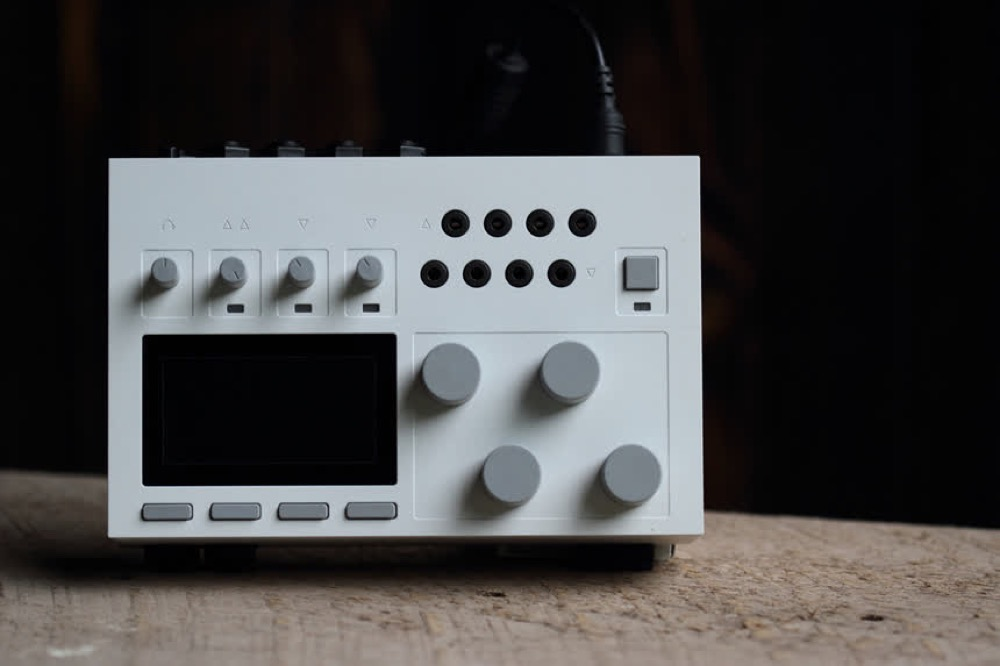
\includegraphics[width=0.75\linewidth,height=0.25\textheight,keepaspectratio]{images/monome-aleph.jpg}
  \caption{monome aleph}
  \caption*{Retrieved from \cite{website-monome-current}}
  \label{fig:monome-aleph}
\end{figure}

The aleph had a focus on community building by releasing the technical documentation and guides for enthusiasts to write and share their own extensions of the software, written in the C programming language. Even though monome only made 100 units of the aleph, it directly influenced their next sound computer, norns, currently available both as an instrument and a \acrshort{DIY} shield for the Raspberry Pi computer.

\begin{figure}[ht]
  \centering
  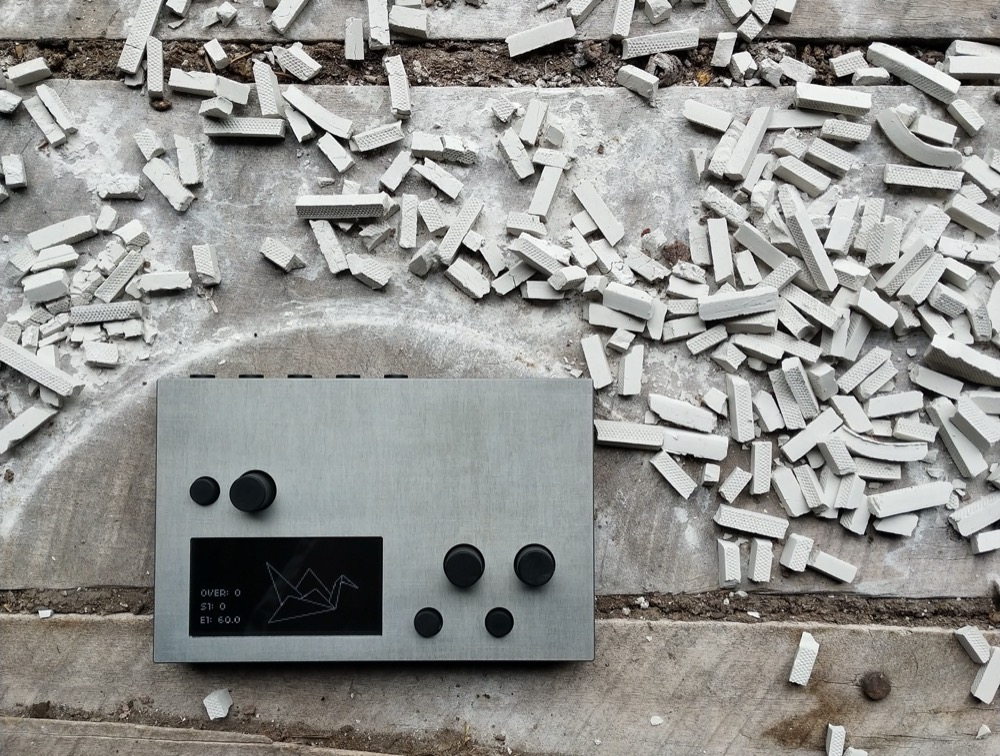
\includegraphics[width=0.75\linewidth,height=0.25\textheight,keepaspectratio]{images/monome-norns.jpg}
  \caption{monome norns}
  \caption*{Retrieved from \cite{website-monome-current}}
  \label{fig:monome-norns}
\end{figure}

The norns runs the Linux operating system, uses SuperCollider for sound generation, and runs Lua scripts for other tasks, such as reading the data from the buttons and encoders, displaying visuals on the screen, and sharing variables with the sound engine. Users are encouraged to write their own software in these two languages, and there is a strong community, both at monome's forum \url{https://norns.community/} and at the norns wiki \url{https://norns.community/}.

\subsection{Shbobo}

In my first semester at MIT, I was introduced by classmate Will Freudenheim \cite{website-will-freudenheim}  to the Shbobo Shnth synthesizer by Peter Blasser. The Shnth is a microcontroller-based scriptable instrument, with multiple input sensors, including flex sensors,  a microphone, and capacitive skin proximity.

\begin{figure}[ht]
  \centering
  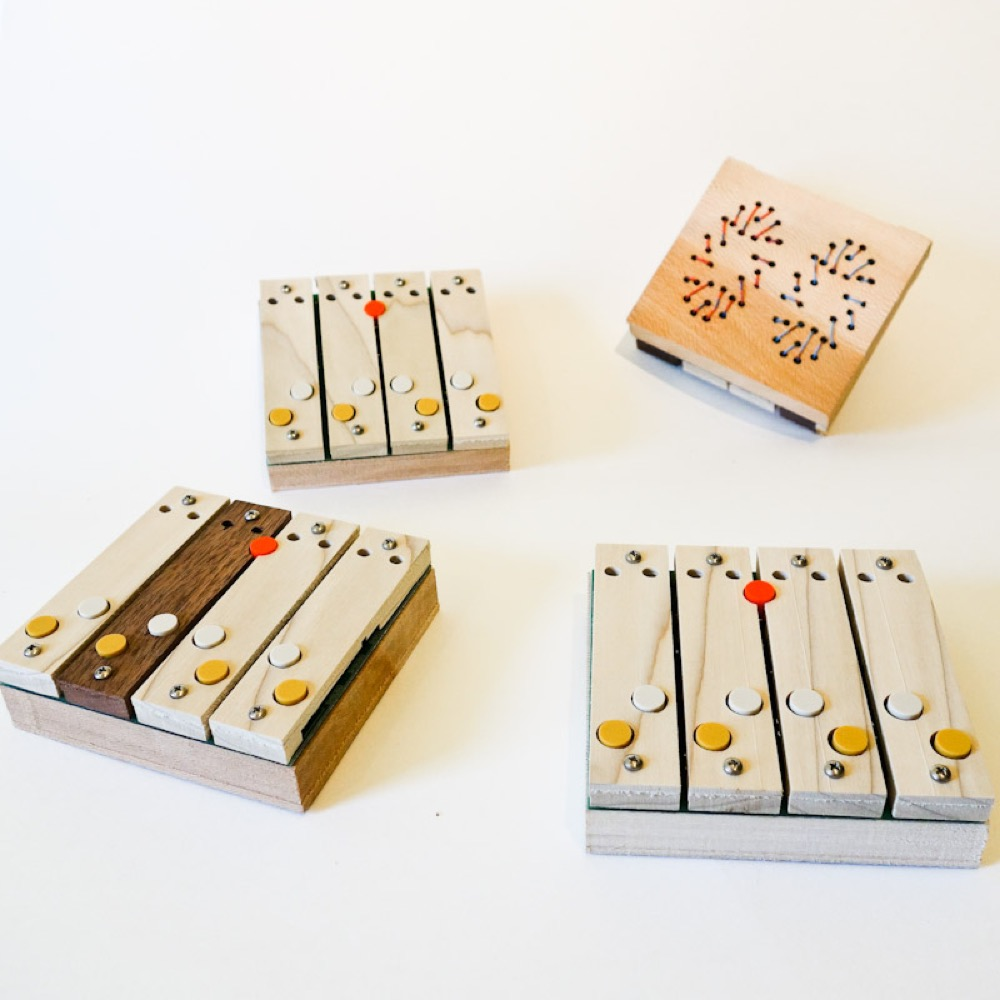
\includegraphics[width=0.75\linewidth,height=0.25\textheight,keepaspectratio]{images/shbobo-shnth.jpg}
  \caption{Shbobo Shnth}
  \caption*{Retrieved from \cite{website-shbobo-current}}
  \label{fig:shbobo-shnth}
\end{figure}

Peter Blasser is an instrument maker, dedicated to \gls{synthesynthesis}, the synthesis of synthesizers \cite{blasser2015stores}. Peter has created several companies of musical instruments, each one of them with different features and philosophies. The most famous one is Ciat-Lonbarde, which use banana cables to make connections between their jacks, for sharing audio and control signals. Another companies include Tocante, with a line of solar-powered touch-based instruments, and Ieaskul F. Mobenthey, a line of Eurorack modules.

For this thesis I want to focus on the company Shbobo, a digital collection of instruments based on microcontrollers, which is made up of the already mentioned Shnth, and the Shtar, a 17-fret string instrument.

\begin{figure}[ht]
  \centering
    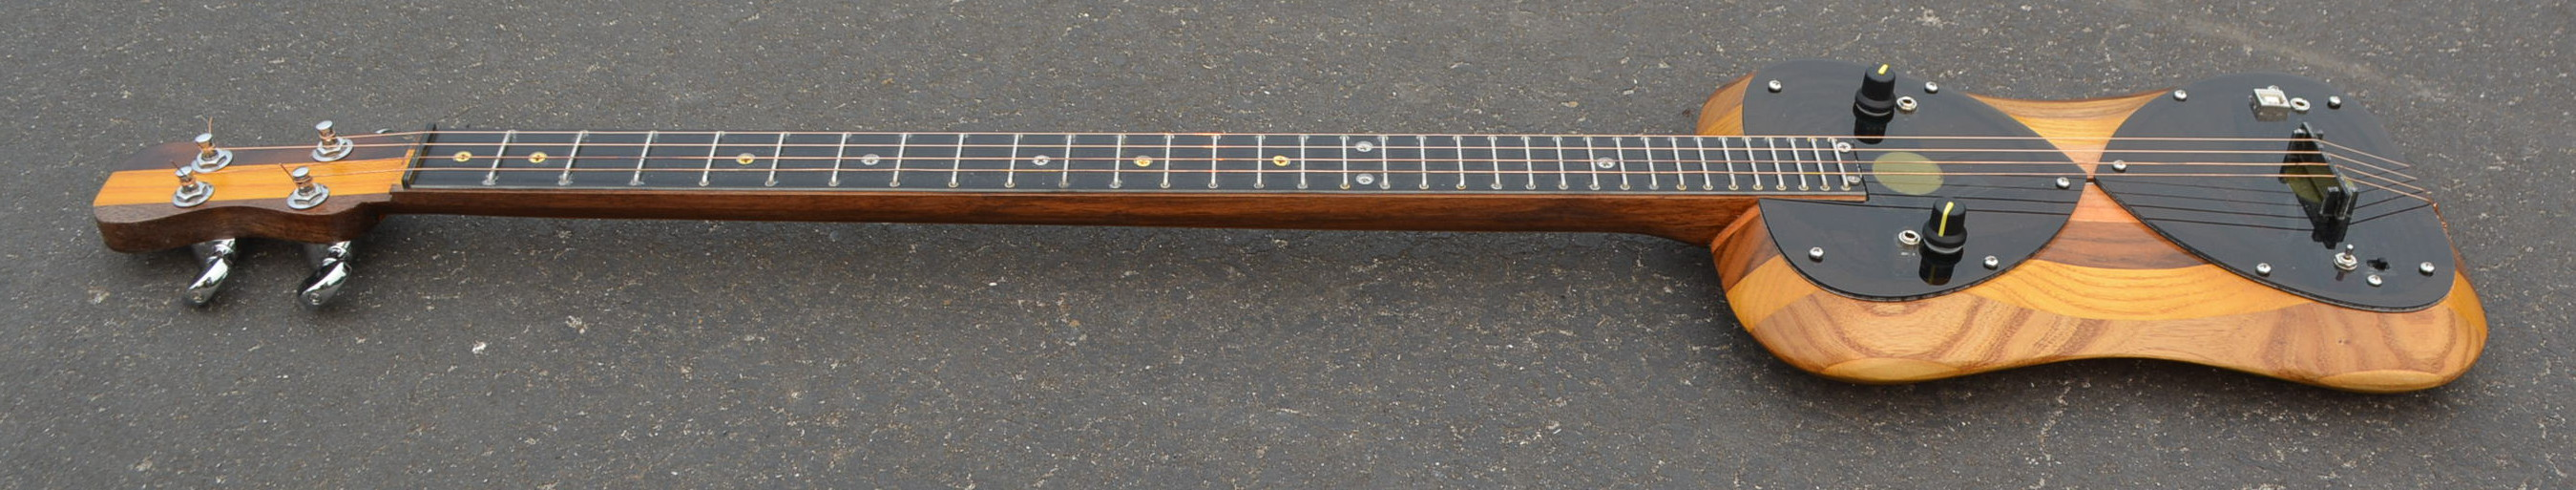
\includegraphics[width=0.75\linewidth,height=0.25\textheight,keepaspectratio]{images/shbobo-shtar.jpg}
  \caption{Shbobo Shtar}
  \caption*{Retrieved from \cite{website-shbobo-current}}
  \label{fig:shbobo-shtar}
\end{figure}

Both the Shnth and the Shtar can be programmed using an open source language called Shlisp, available at \url{https://github.com/pblasser/shbobo}. The Shlisp language allows the use of different sensors on the instruments to control different oscillators, filters, and effects, and interactions between the sound engine and the instrument interface. Just like all of the instruments by Peter Blasser, the Shbobo instruments don't follow classical Western musical conceptions of notes and scales, but rather follow the approach of pioneers such as Don Buchla, by making their own language for describing the instruments' behavior and sounds.

They promote computer-centric approaches to making sound, such as the use of integers and metaphors of finite state machines, and also allow for different ways of playing and sensing, such as the use of antennas for detecting hand distance, a microphone for detecting speech and whistling, and wooden bars with piezos for detecting pressure.

\section{Education}

This thesis is also inspired by the work of the research group Lifelong Kindergarten at the MIT Media Lab, led by professor Mitchel Resnick. In the book with the same title, he builds on Seymour Papert’s work and proposes that educational projects should have “Low floor, wide walls, high ceilings.” Additionaly, that learners thrive when they engage in the 4 Ps: “Projects, passion, peers, and play.”

In terms of projects, this thesis includes the release of a software library, so that people can make the software their own, and spin off their own projects. It is also open source so that people can learn from my mistakes and also \gls{fork} to adapt to their needs.

In terms of passion, this thesis is a contribution to the ecosystem of instrument makers, so that other people can enjoy my same passion, of making art with computation.

In terms of peers, I have been lucky to have been supported by the MIT UROP office and MIT Media Lab, and had the opportunity to work with MIT undergrad researchers Peter Tone and Maxwell Wang. Also, this project was taught in collaborative workshops where people could discuss their ideas with their peers.

In terms of play, this thesis project is not about correct answers, or even excellent classification with \acrshort{ML}, it's all about finding innovative ways to interact with multimedia material, celebrate the small victories and the big glitches, and iterate over and over again.

\section{Digital rights}


So far I have felt comfortable doing scraping in private, for academic or artistic purposes, but not for more public or commercial outlets. For Tiny Trainable Instruments, I was worried about including web scraping techniques, because I didn't want to infringe any copyrights or be involved in litigation.

Because of my concerns, I reached out to the Technology Law Clinic \cite{website-boston-university-technology-law-clinic} at Boston University's School of Law. My request was for them to assess the potential civil and criminal liabilities if I conducted web scraping on Youtube.com, in order to to train my machine learning algorithms. I also inquired about the legal implications of publishing my databases, my trained models, and related tutoria for encouraging other people to also do web scraping.

The Technology Law Clinic gave me a breakdown of the legal risks associated with web scraping, and they confirmed with me that I could be in violation of three different laws: the \acrfull{CFAA}, the \acrfull{DMCA}, and the Copyright Act. This confirmation cemented my decision of using the Arduino microcontroller as a source for my data, so that all my databases would be homemade and fully original. I hope my contributions in how to capture data, parse it, and how to use it to build your own databases is also helpful to others.

I am no expert on digital or human rights at all, but I am convinced that it's a human right to not be surveilled, and I hope this thesis helps to illustrate different strategies I have learned while at MIT. During my research and my class with Sasha Costanza-Chock, I studied or became aware of different efforts in programming for activism, including the Guardian Project by the Electronic Frontier Foundation, which made me decide to include privacy and consent as key topics on this project.

Since \acrshort{ML} algorithms need data to be trained on, and corporations and governments are hungry about gathering our data, it is of critical importance for this decade for people to be aware of the pitfalls and dangers of algorithmic bias and surveillance, and I think the techniques, documentation, and proposals I make for building custom databases for this project, help in the educational efforts for society's safe practices around their data.

I am constantly in awe of the work by countless activists, including Edward Snowden, Joy Buolamwini, and Chelsea Manning, who have spoken truth to power.

\section{Opera of the Future research projects}

During the development of this thesis, I have been fortunate to collaborate on different capacities with other thesis projects by classmates at the Opera of the Future research group, which has directly inspired my work.

\subsection{Squishies, by Hannah Lienhard}

Squishies is Hannah Lienhard's Master's thesis, and consists of novel squishable interfaces for musical expression. We shared discussions about low-level sound design, code reusability, sound art education, and digital instruments. We were part of a Master's thesis working group, facilitated by Roya Moussapour with two other Media Lab classmates, where we workshopped drafts of our thesis. This practice and feedback has been critical in shaping the language and discourse of this thesis document.

\subsection{Fluid Music, by Charles Holbrow}

Fluid Music is Charles Holbrow's PhD thesis. It is a software framework for music composition and produciont. The design of the interface, documentation, and scope of Charles' thesis were a direct influence on the documentation and API coding style of this project. I was fortunate to collaborate with Charles, by testing the software library, discussing documentation design, and participating in one of his workshops teaching with Fluid Music, which in turn inspired me to include my own workshop for user feedback and release of this project.
